Podemos considerar a la World Wide Web (más comúnmente conocida como sólo Web) como una colección de páginas web (documentos) la cual crece y cambia día a día. En este capítulo se desarrollan conceptos sobre cómo tratar a la Web, al ser tan diferente de todos las colecciones tradicionales anteriormente vistas.

\section{Historia}
	Como bien se detalló anteriormente, la Web no tiene precedentes en diversas cuestiones:
	\begin{itemize}
		\item En escala.
		\item En la falta de coordinación a la hora de su desarrollo.
		\item En la diversidad de sus participantes.
	\end{itemize}
	Esto hace que recuperar información en la Web sea más complicado que recuperar información en colecciones de documentos tradicionales. \par
	
	Veamos, de forma resumida, cómo es el funcionamiento de comunicación entre un \textit{cliente} y un \textit{servidor}:
	\begin{quotation}
		Un \textit{cliente} (tal como un \textit{browser}; es decir, una aplicación con interfaz gráfica que renderiza el contendido de código HTML) envía un pedido a un servidor web. El \textit{browser} especifica una URL (\textit{Universal Resource Locator}) como, por ejemplo \texttt{http://www.google.com.ar/intl/en/policies/terms/regional.html}. En el ejemplo anterior, la cadena de caracteres \texttt{http} refiere al protocolo que se debe usar para transmitir datos (HTTP, por \textit{HyperText Transfer Protocol}). La cadena de caracteres \texttt{google.com.ar} refiere al dominio y especifica la raíz de la jerarquía de páginas web. \texttt{/intl/en/policies/terms/regional.html} indica la ruta en donde se encuentra el archivo HTML \texttt{regional.html} que es el cual, al fin y al cabo, será retornado por el servidor web que se encuentra en \texttt{www.google.com.ar} y es con el cual el \textit{cliente} interactuará. En este archivo, también, se encuentran los \textit{links}. Este procedimiento es clave a la hora de obtener el contenido de una página web (texto y \textit{hyperlinks}) para indexar documentos
	\end{quotation}
	
	El hecho de que los \textit{browsers} fueron y son capaces de mostrar al usuario el código HTML detrás de una página web, hizo que muchos developers y aspirantes desarrolladores de páginas web, aprendieran cómo estaban implementadas aquellas páginas que consideraban modelos y, así, implementaran las suyas. De esta manera, el número de páginas web en la Web comenzó a incrementar y a convertirse en un espacio en donde cualquier persona, con algunos pocos conocimientos informáticos, pudiese comunicarse y expresarse ante millones de personas alrededor del planeta. De repente, la Web se convirtió en la mejor opción a la hora de obtener y proveer información. \par
	
	Toda la información que contiene la Web es inservible si no se posee herrmientas para descubrir y recuperar información. Y, lo más importante, que éstas herramientas estén al alcanze de usuarios \textit{comunes} que navegan la web a través de un web \textit{browser}; es decir, éstas herramientas deben ser lo más simples posibles. Por lo tanto, los primeros científicos e investigadores tomaron noción de la desventaja anterior y comenzaron a desarrollar los primeros buscadores web. Los primeros intentos se podían dividir en dos categorías:
	\begin{itemize}
		\item Motores de búsquedas de indexación de texto tales como Altavista, Excite y Infoseek. Consistía en consultas escritas en lenguaje natural (o en uno cercano al mismo) utilizando índices invertidos y mecanismos de \textit{ranking} tales como se detalló en capítulos anteriores.
		\item Utilizando taxonomías. En éste caso, se le presentaba al usuario un \textit{árbol} jerárquico el cual él mismo debía recorrer hasta llegar a la página deseada. Esto tiene grandes desventajas, veamos:
			\begin{itemize}
				\item Clasificar páginas web en categorías es, prácticamente, un trabajo manual. Por lo tanto, es difícil de escalar con el tamaño de la Web.
				\item Sólo se deben categorizar las \textit{mejores} páginas web y dejar de lado las demás. Ahora, ¿qué se considera como una \textit{buena} página web?.
			\end{itemize}
	\end{itemize}
	Dadas las desventajas anteriores, la popularidad de las taxonomías disminuyó con el tiempo. Una de las grandes empresas que las implementaba en su buscador era Yahoo!. \par
	
	Como se detalló anteriormente, implementar buscadores web utilizando taxonomías era \textit{exponencialmente} ineficiente. Por lo tanto, se siguió estudiando cómo utilizar las técnicas de recuperación de información tradicionales; es decir, aquellas que implementan índices invertidos y funciones de relevancia para ordenar documentos, teniendo en cuenta el gran volúmen de documentos en la Web. Los primeros motores de búsqueda contenía índices conteniendo millones de documentos. Estos fueron satisfactorio en cuanto a indexar una gran parte de la Web en ese momento, pero no eran eficiente a la hora de ordenar documentos por relevancia. Por lo tanto, para controlar la calidad de las páginas se necesitaron nuevos mecanismos y técnicas de recuperación de información, aunque basados en la teoría tradicional de sistemas de recuperación de información.
	
\section{Características de la Web}
	Publicar en la Web se convirtió en un medio de democratización disponible para millones de personas. Con lo cual, crear contenido, ahora, no solo es tarea de editores bien entreanados sino también de millones de personas con acceso a Internet. Esto conlleva a preguntarse en cuánto podemos confiar en el contenido disponible en diversas páginas web. La democratización, como bien se detalló anteriormente, de la creación de contenido convirtió rápidamente a la Web como un medio el cual contiene verdades, mentiras y contradicciones. De lo anterior, nace la siguiente pregunta: \textit{¿en qué páginas debemos confiar?}. Esta es una pregunta difícil de responder ya que para ciertas personas, algunos editores pueden ser confiables como otros pueden no serlo. Cómo un motor de búsqueda en la Web debe computar esta medida de \textit{confianza} a cada página web es lo que se busca desarrollar a lo largo de éste capítulo. Esto es de suma importancia ya que, para los usuarios finales de la Web, un motor de búsqueda es la única vía para recuperar información entre miles de millones de documentos disponibles.
	
\subsection{\textit{Web Graph}}
	Según \cite{manning2009}, podemos dividir las páginas web en \textbf{estáticas} o \textbf{dinámicas}. Se consideran estáticas aquellas las cuales su contenido no varía de un pedido para ésa página a la siguiente. Un profesor que manualmente mantiene su propia página web, se considera estática. Mientras que las dinámicas son mecánicamente generadas por una aplicación que reside en un servidor en respuesta a una consulta a una base de datos (una señal de tales páginas web son las cuales, en sus URLs, poseen el signo \texttt{?}). \par
	
	Sabemos que para definir un grafo, debemos definir su conjunto de nodos y aristas; luego, \cite{manning2009} define al \textit{web graph} de la siguiente forma:
	\begin{itemize}
		\item El conjunto de nodos es igual al conjunto de todas las páginas web HTML estáticas pertenecientes a la Web.
		\item Se considera como una arista dirigida a todo \textit{hyperlink} que \enquote{conecta} una página web a otra página web.
	\end{itemize}
	El \textit{web graph} no es fuertemente conexo: existen pares de páginas web las cuales es imposible proseguir desde una página del par hacia la otra siguiendo \textit{hyperlinks}. Se definen como \textbf{in--links} a aquellos \textit{hyperlinks} que \enquote{salen} desde una página web y \textbf{out--links} a aquellos que \enquote{llegan} a una página web.
	
	%% figura 19.3 de manning2009
	\begin{figure}[h]
		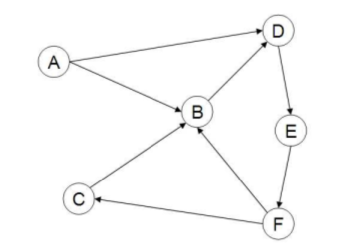
\includegraphics[width=8cm]{small-web-graph}
		\centering
		\caption{\textit{Web graph} en el cual existen seis páginas web. La página web posee 3 \textit{out--links} y 1 \textit{in--link}}
	\end{figure}
	
\section{La experiencia de usuario en un buscador web}
	Como se ha descrito anteriormente, la búsqueda de información en la Web cambia de forma significante con respecto a los sistemas de recuperación tradicionales vistos. En éstos últimos, los usuarios debían ser profesionales en el arte de la búsqueda de informacion; es decir, científicos de la información: debían tener entrenamiento desde cómo escribir una consulta (por ejemplo, una consulta \textit{booleana} si se trataba de un modelo de recuperación booleano) hasta tener un buen conocimiento en cómo estaban estructurados los documentos dentro de la colección. En contraste, los usuarios de sistemas de recuperación de información en la Web tienden a no saber e importar cómo los documentos (páginas web) están estructurados y cómo se debe escribir una consulta. En resúmen, los motores de búsqueda en la Web no deben imponer éstas restricciones ya que, al fin y al cabo, sus usuarios no son profesionales en la búsqueda de información. \par
	
	Claramente, cuanto más tráfico un motor de búsqueda en la Web pueda atraer, tendrá más ganancia económica con respecto a las búsquedas patrocinadas. Por lo tanto, ¿cómo hacen los motores de búsquedas para lograr lo anterior?. Del gran éxito de Google, podemos aprender lo siguiente:
	\begin{itemize}
		\item Enfoque en \textit{precisión} en vez de en \textit{recall} en los primeros resultados.
		\item Interfaz gráfica de usuario simple, liviana y con pocos elementos gráficos. Es decir, una interfaz en donde el texto sea el elemento gráfico más importante. Esto hace que la experiencia sea totalmente \textit{responsive} y no esperar demasiado tiempo en cargar los resultados de la búsqueda.
	\end{itemize}
	
	Ahora, según \cite{manning2009}, las consultas que los usuarios pueden realizar, en un buscador web, pueden tener diversos propósitos y se pueden clasificar en los siguientes tres:
	\begin{itemize}
		\item \textit{Consultas de información}. Son aquellas las cuales buscan recuperar información sobre algún tema en particular (como por ejemplo, cáncer) y, en general, no existe una única página web la cual contiene toda la información necesaria.
		\item \textit{Consultas de navegación}. En éstas, los usuarios buscan la página web oficial de alguna entidad (por ejemplo, Apple): esperan que el primer resultado que devuelva el motor de búsqueda resulte ser la mismísima página de la entidad en cuestión. Suele suceder que el usuario no esté buscando más información sobre la entidad; es decir, no le interesa otros documentos que no sean el \textit{homepage} oficial.
		\item \textit{Consultas de transacción}. El objetivo de toda consulta de transacción es realizar una transacción, de algún tipo, en la Web: tales como comprar un producto, descargar un archivo, realizar una reserva y demás. En éstos casos, el usuario espera que el motor de búsqueda retorne páginas web que realicen los servicios antes mencionados.
	\end{itemize}
	
	Decidir en cuál categoría subyace una determinada consulta puede ser un gran reto.
	
\section{\textit{Web crawling}}
	\subsection{Introducción}
		\enquote{\textit{Web crawling} es el proceso por el cual se recogen páginas de la Web, con el motivo de indexarlas y soportar un motor de búsqueda}, \cite{manning2009}. Su objetivo es recoger el número máximo de páginas útiles, junto con la estructura de \textit{links} que las interconectan, de forma rápida y eficiente. \par
		
		El foco de ésta sección es detallar el funcionamiento de un \textit{web crawler}, también a veces llamado \textit{web spider}.
		
		%% figura 19.7 (manning2009) 
		
	\subsection{Características que un \textit{crawler} debe proporcionar}
		\begin{itemize}
			\item \textbf{Robustez}. En la Web, existen servidores los cuales crean los denominados \textit{spider traps}; éstos son generadores de páginas web que engañan a los \textit{crawlers} logrando que los últimos extraigan información de infinitas páginas web dentro de un determinado dominio. Luego, los \textit{crawlers} deben ser lo suficientemente inteligentes como para sortear los \textit{spider traps}. Cabe destacar que no siempre éstas \enquote{trampas} son maliciosas: muchas veces son el resultado de carencia de profesionalismo en el desarrollo de páginas web.
			\item \textbf{Cortesía}. Los servidores web especifícan de forma implícita y también explícita políticas las cuales regulan cada  \enquote{cuánto} un \textit{crawler} puede visitarlos. Estas políticas se deben respetar.
		\end{itemize}
	
	\subsection{Características que un \textit{crawler} debería proporcionar}
		\begin{itemize}
			\item \textbf{Distribución}. El \textit{crawler} debería tener la posibilidad de ejecutarse en máquinas distribuidas.
			\item \textbf{Escalable}. La arquitectura del \textit{crawler} debería ser lo más práctica posible como para poder extenderse y escalar su frecuencia de rastreo añadiendo más hardware y ancho de banda.
			\item \textbf{\textit{Performance} y eficiencia}. El sistema de \textit{crawling} debería utilizar de forma eficiente recursos de sistemas como ancho de banda, procesador, almacenes de datos, y demás.
			\item \textbf{Calidad}. El \textit{crawler} debería procesar, primero, aquellas páginas de la Web que sean \enquote{útiles}.
			\item \textbf{Frescura}. Aquellas páginas web las cuales son devueltas por un motor de búsqueda deberían estar actualizadas. Por lo tanto, el \textit{crawler} debe procesar páginas con una frecuencia que se aproxime a la frecuencia con la cual páginas web modifiquen su contenido.
			\item \textbf{Extensibilidad}. La aquitectura de los \textit{crawlers} deberían ser modulares. Esto permite que éstos puedan adaptarse con nuevas tecnologías de datos, nuevos protocolos de extracción de información, y demás.
		\end{itemize}
		
	\subsection{Funcionamiento de un \textit{crawler}}
		Veamos en qué consiste el funcionamiento básico de un \textit{web crawler}. El \textbf{crawler} comienza con un conjunto inicial, también llamado \textit{conjunto semilla}, que contiene una o más URLs. Toma una URL de éste conjunto, extrae el texto y sus \textbf{links} (los cuales apuntan a otra página web). El texto que se extrae de cada página web es enviado a un indexador de texto (como hemos analizado en los capítulos anteriores). Las URLs de los \textit{links} que se extrayeron son enviados a un conjunto llamado \textit{frontera de URLs}; el cual contiene URLs los cuales todavía deben ser procesados por el \textit{crawler}. En el comienzo, el conjunto \textit{frontera de URLs} contiene sólo al \textit{conjunto semilla}. La tarea del \textit{crawler} es procesar cada una de las URLs pertenecientes al conjunto \textit{frontera de URLs}. Una vez que dichas URLs son procesadas, son nuevamente colocadas en el conjunto \textit{frontera} con el objetivo de que se extraiga información actualizada de las mismas (ya que, muy probable y razonablemente, el contenido de las páginas web cambie con el tiempo).
		\subsubsection{Arquitectura}
			Un sistema de \textit{crawling} demanda de múltiples módulos, como muestra la Figura \ref{fig:crawler-architecture}. Veamos los más importantes:
			\begin{enumerate}
				\item El conjunto \textit{frontera}, que contiene URLs los cuales aún tienen que ser procesado por el \textit{crawler}.
				\item Un módulo de resolución de DNS el cual, dada una URL, determina el servidor en el cual se encuentra y, por lo tanto, en el cual el \textit{crawler} debe extraer la información.
				\item Un módulo que utiliza el protocolo \texttt{http} para \enquote{devolver} la página web de una determinada URL.
				\item Un módulo que \enquote{parsea} el texto y el conjunto de \textit{links} extraidos de una página web.
				\item Un módulo que determina si un determinado \textit{link} ya ha sido procesado por el \textit{crawler} y si existen \textit{links} duplicados dentro del conjunto \textit{frontera}.
			\end{enumerate}
			
			%% figura 20.1 (manning2009)
			\begin{figure}[h]
				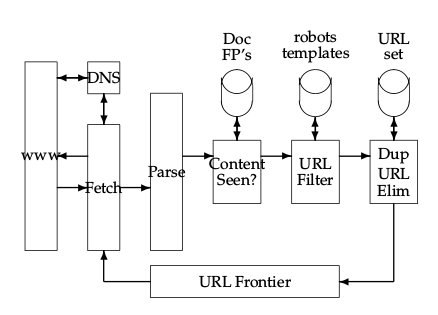
\includegraphics[width=8cm]{crawler-architecture}
				\centering
				\caption{Arquitectura de un web \textit{crawler}}
				\label{fig:crawler-architecture}
			\end{figure}
			
		\subsubsection{\textit{Robots Exclusion Protocol}}
			Muchas veces se quiere que, ciertas páginas de un cierto dominio, no sean alcanzables por un determinado \textit{crawler}; es decir, que éste no las procese. Para realizar ésto, los desarrolladores web (\textit{webmasters}) colocan un archivo, llamado \texttt{robots.txt}, en la raíz de la jerarquía. El protocolo se denomina \textit{Robots Exclusion Protocol}. \par
			
			Veamos un ejemplo de archivo \texttt{robots.txt} el cual especifica que ningún \textit{crawler} (tambíen llamado \textit{agente}) debe visitar ninguna URL cuya posición en el archivo de jerarquía comienza con \texttt{/yoursite/temp}, excepto por el \textit{crawler} \enquote{searchengine}:
			\begin{quote}
				\begin{ttfamily}
					User-agent: * \\
					Disallow: /yoursite/temp/ \\ \\
					
					User-agent: searchengine \\
					Disallow:
				\end{ttfamily}
			\end{quote}
			
			Este archivo debe ser extraido desde el sitio web con el fin de comprobar si la URL en cuestión satisface las restricciones, y puede, por lo tanto, ser añadida al conjunto \textit{frontera de URLs}.
			

\section{Análisis de \textit{links}}
	Dada una consulta de usuario en un buscador web, éste debe ordenar (crear un \textit{ranking}) en orden de \enquote{imporancia} las páginas web que obtiene como resultado. Una de las técnicas comúnmente usadas por sistemas de recuperación de información en la Web es llamada \enquote{análisis de \textit{links} }, cuyo objetivo es computar un puntaje a una página web dada cualquier consulta. \par
	
	El análisis de \textit{links} está \enquote{inspirado} en el análisis de citación, el cual se utiliza en el área conocida como bibliometría. El análisis de citación busca, resumidamente, cuantificar la influencia (\enquote{importancia}) de artículos escolares analizando el patrón de citaciones entre ellos. El análisis de \textit{links} en la Web trata a los \textit{hyperlinks} que lleva de una página web hacia otra página web como una \enquote{atribución de autoridad}; es decir, si una página $A$ desarrolla un tema en particular y añade un \textit{link} $l$, para obtener más información sobre el tema, el cual apunta a otra página web $B$, implícitamente, la página $A$ le concede autoridad sobre el tema en cuestión a la página $B$. \par
	
	Cabe destacar que, simplemente reconocer la importancia de una página web mediante el número de \textit{in-links} 	que posee no es buena idea: por ejemplo, personas mal intencionadas pueden crear otras páginas conteniendo \textit{links} que apunten a una página en particular la cual se quiere que obtenga más relevancia para ubicarse en los primeros puestos en respuesta a determinadas búsquedas en la Web. El ejemplo anterior se conoce como \textit{link spam}. \par
	
	En ésta sección se desarrollará ideas básicas sobre el uso del \textit{web graph} en el análisis de \textit{links}. Se detallará un método de análisis de \textit{links} en particular: PageRank.
	
	\subsection{Conceptos básicos}
		La siguiente figura representa dos páginas web $A$ y $B$ donde, en $A$, existe un \textit{link} el cual apunta a $B$. El análisis de \textit{links} se basa en dos conceptos:
		\begin{enumerate}
			\item El \textbf{anchor text} que apunta a la página $B$ es una buena descrpción sobre qué trata $B$.
			\item El \textit{link} de $A$ hacia $B$ representa una \enquote{ratificación} de la página $B$, por el creador de $A$. Esto no siempre ocurre; por ejemplo, muchas páginas web de empresas poseen, en cada página de su dominio, punteros (\textit{links}) hacia notas de copyright. El análisis de \textit{links} descarta aquellos \textit{links}.
		\end{enumerate}
		
		%% figura 19.2 (manning2009)
		
		Veamos el siguiente \textit{link}, el cual apunta a la página web del \textit{Journal of the ACM}:
		\begin{quote}
			\begin{ttfamily}
				<a href="http://www.acm.org/jacm/">Journal of the ACM</a>
			\end{ttfamily}
		\end{quote}
		En éste, su correspondiente \textit{anchor text} es \textit{Journal of the ACM} y, claramente, describe el contenido de la página web \texttt{http://www.acm.org/jacm/}. \par
		
		El uso de \textit{anchor texts} puede ser explotado por motores de búsqueda. Por ejemplo, los términos de los \textit{anchor texts} pueden ser incluidos como términos bajo los cuales indexar la página web destino, indicando que éstos términos ocurren como \textit{anchor texts} en lugar de términos dentro de la página. Por lo tanto, los \textit{postings} para el término \texttt{computer} incluirá el documento \texttt{http://www.ibm.com}, \texttt{http://www.apple.com}, entre otros. \par
		
		Los \textit{anchor texts}, también, pueden utilizarse para producir \textit{spam}: un página web puede autoreferenciarse creando \textit{anchor texts} apuntando a si mismo para lograr más relevancia ante ciertas consultas de términos. Este tipo de \textit{spam} es combatido y detectado por motores de búsqueda.
		
	\subsection{PageRank}
		PageRank es un método de análisis de \textit{links} introducido por Google. El objetivo de éste método es asignar a cada página web del \textit{web graph} un puntaje numérico entre 0 y 1. A éste puntaje se lo conoce como su \textit{PageRank}. El PageRank de un nodo dependerá de la estructura de \textit{links} del \textit{web graph}. Un motor de búsqueda, dado una consulta, computa para cada página web un puntaje el cual es la combinación de cientos de métodos como la similitud del coseno y proximidad de términos, junto con el puntaje que otorga el método PageRank. \par
		
		Idea:
		\begin{quote}
			\begin{itshape}
				\enquote{Consideremos un usuario de la Web que comienza en una determinada página (un nodo del web graph) y comienza una caminata aleatoria, en la Web, como sigue. En cada paso, el usuario procede desde su actual página web A hacia otra página B, elegida aleatoriamente, la cual A apunta mediante un hyperlink. La Figura \ref{fig:random-surfer} muestra al usuario en el nodo A. A contiene tres hyperlinks los cuales apuntan a sus respectivas páginas web B, C y D. En el siguiente paso, el usuario procede a alguno de éstos tres nodos con probabilidad equivalentes 1/3. Mientras el usuario continúa la caminata, visitará más frecuentemente algunos nodos a comparación de otros. Intuitivamente, éstas son páginas web con un número mayor de \textbf{in--links} que otras. La idea de PageRank es que los nodos los cuales, durante ésta caminata, son frecuentemente más visitados que otros son más importantes}
			\end{itshape}, \cite{manning2009}.
		\end{quote}
		
		%% Figura 21.1 (manning2009)
		\begin{figure}[]
			\centering
			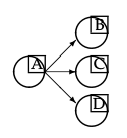
\includegraphics[width=3cm]{random-surfer}
			\caption{Un usuario aleatorio de la Web quien se encuentra en la página A.}
			\label{fig:random-surfer}
		\end{figure}
		
		
		Ahora, podemos encontrarnos con el problema en el cual el usuario se encuentra en un determinado nodo del \textit{web graph} el cual no posee \textit{out--links}. Para resolver éste problema, el método PageRank introduce una operación llamada \textit{teleport}. En ésta, el usuario \enquote{salta} desde un nodo hacia otro en el \textit{web graph}. La operación se lleva a cabo porque el usuario escribe otra URL en el \textit{browser}. Si $N$ es el número total de nodos en el \textit{web graph}, \textit{teleport} lleva al usuario a todos los nodos con probabilidad 1/$N$. \par
		
		Cuando se asigna el puntaje PageRank a cada nodo del grafo, se utiliza la operación \textit{teleport} de dos maneras:
		\begin{itemize}
			\item Cuando un nodo no contiene \textit{out--links}, el usuario invoca la operación \textit{teleport}.
			\item Cuando un nodo contiene \textit{out--links}, el usuario invoca la operación \textit{teleport} con probabilidad $0 < \alpha < 1$ y la caminata estándar anteriormente detellada con probabilidad $1 - \alpha$, donde $\alpha$ es un parámetro anteriormente elegido (por lo general, $\alpha = 0,1$).
		\end{itemize}
		
		Veremos que en el proceso combinado (caminata aleatoria más invocación de la operación \textit{teleport}) que realiza el usuario al nevegar por la Web, éste visita cada nodo $v$ del \textit{web graph} una fracción fija de tiempo $\pi (v)$ la cual depende de la estructura de \textit{links} del \textit{web graph} y el valor anteriormente fijado de $\alpha$. Al valor $\pi (v)$ se lo llama \textit{PageRank} de $v$. Ahora, para poder computar éste valor debemos recordar algunos conceptos como, por ejemplo, cadenas de Markov.
		
		\subsubsection{Cadenas de Markov}
			Definición:
			\begin{quote}
				En la teoría de la probabilidad, se conoce como cadena de Markov a un tipo especial de proceso estocástico discreto en el que la probabilidad de que ocurra un evento depende \textit{solamente} del evento inmediatamente anterior. Esta propiedad recibe el nombre de \textit{propiedad de Markov}.
			\end{quote}
			
			Una cadena de Markov consiste de $N$ \textit{estados} (eventos). Para hacer una analogía con el \textit{web graph}, cada estado en una cadena de Markov corresponderá a una página web (nodo) del mismo. \par
			
			La representación de una cadena de Markov se realiza mediante una matriz $N \times N$ llamada \textit{matriz de probabilidades de transición}, la cual notamos como $P$. En ésta, se cumplen las siguientes propiedades:
			\begin{itemize}
				\item $P_{i,j} \in [0,1], \forall i,j$, y
				\item $\sum_{j = 1}^{N} P_{i,j} = 1, \forall i$.
			\end{itemize}
			La cadena de Markov puede estar en cualquiera de los $N$ estados en cualquier momento. $P_{i,j}$ nos indica la probabilidad de que la cadena de Markov, en el siguiente paso, se encuentre en el estado $j$, dado que el estado actual es $i$. Este valor se conoce como \textit{probabilidad de transición} y sólo depende del estado actual $i$. \par
			
			Veamos un ejemplo en el cual tenemos una cadena de Markov con tres estados: $A$, $B$ y $C$. En ésta, desde el estado $A$ se puede proseguir con una probabilidad de 0.5 al estado $B$ ó al estado $C$. Desde $B$ o $C$, es posible proseguir con probabilidad 1 al estado $A$. \par
			
			%% Figura 21.2 (cadena y matriz) (manning2009)
			\begin{figure}[]
				\centering
				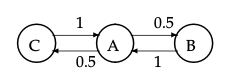
\includegraphics[width=4cm]{markov-chain}
				
				\[
			P =
			\begin{bmatrix}
				0 & 0.5 & 0.5 \\
				1 & 0 & 0 \\
				1 & 0 & 0
			\end{bmatrix}
			\]
			
				\caption{Cadena de Markov}
			\end{figure}
			
			Un \textbf{vector de probabilidad} $N$--dimensional en el cual cada componente corresponde a uno de los $N$ estados de una cadena de Markov puede ser visto como la distribución de probabilidades sobre sus estados. La suma de los $N$ componentes del vector debe ser 1. \par
			
		\subsubsection{Utilizando cadenas de Markov en el \textit{web graph}}
			Ahora, ¿cómo podemos utilizar la teoría de la probabilidad, más específicamente cadenas de Markov, para modelar la actividad de un usuario al \enquote{navegar} por la Web?. Podemos pensar a un usuario aleatorio que navega por el \textit{web graph} como una cadena de Markov, con un estado por cada página web, y cada transición de probabilidad siendo representada por la probabilidad de moverse desde una página web hacia otra. Como es de esperar, \textbf{la operación \textit{teleport}} vista anteriormente, \textbf{contribuye en la obtención de éstas probabilidades de transición}. Notemos $A$ a la matriz de adyacencias correspondiente al \textit{web graph}; es decir, si existe un \textit{link} desde la página $i$ hacia la página $j$, entonces $A_{i,j} = 1$, en caso contrario $A_{i,j} = 0$. Como útimo paso, debemos crear la matriz de probabilidades de transición $P$ para nuestra cadena de Markov. Podemos derivar, muy simplemente, $P$ de $A$ aplicando el siguiente algoritmo:
			\begin{enumerate}
				\item Si una fila de $A$ no tiene 1's, luego reemplar cada elemento de la fila por 1/$N$. Para todas las demás filas proceder como sigue.
				\item Dividir cada 1 en la matriz $A$ por el número de 1's en su fila.
				\item Multiplicar la matriz resultante por $1 - \alpha $.
				\item Sumar $\alpha /N$ a cada elemento de la matriz resultante, para obtener finalmente la matriz $P$.
			\end{enumerate}
			
			\begin{quote}
				\textbf{Ejemplo 8.1} Para entender un poco mejor el algoritmo anterior, veamos un ejemplo. Consideremos un \textit{web graph} con tres nodos 1, 2 y 3, y los \textit{links} están definidos como siguen: $1 \rightarrow 2$, $3 \rightarrow 2$, $2 \rightarrow 1$, $2 \rightarrow 3$. \\
				La matriz de adyacencias, $A$, es la siguiente:
				\[
				A =
				\begin{bmatrix}
					0 & 1 & 0 \\
					1 & 0 & 1 \\
					0 & 1 & 0
				\end{bmatrix}
				\]
				
				Finalmente, una vez aplicado el algoritmo anterior, obtenemos la matriz de transición de probabilidades $P$:
				\[
				P =
				\begin{bmatrix}
					1/6 & 2/3 & 1/6 \\
					5/12 & 1/6 & 5/12 \\
					1/6 & 2/3 & 1/6
				\end{bmatrix}
				\]
			\end{quote}
			
			Podemos representar la probabilidad de distribución de la caminata de un usuario en la Web, en cualquier momento, mediante el vector de probabilidades $\vec{x}$. Razonablemente, cuando $t = 0$ (es decir, al comienzo de la caminata del usuario en la Web), el usuario comenzará en aquel estado $s$ el cual $\vec{x}_s = 0$ y para todo estado $j \neq s$, $\vec{x}_j \neq 0$. Por definición, la distribución de probabilidades de la caminata de un usuario cuando $t = 1$ está dada por el vector de probabilidades $\vec{x}P$; cuando $t = 2$ por $(\vec{x}P)P = \vec{x}P^{2}$, y así sucesivamente. Por lo tanto, podemos calcular la probabilidad de distribución de la caminata en la Web de cualquier usuario en cualquier momento con tan solo el vector de distribuición inicial (es decir, aquel el cual indica en qué página web comienza el usuario) y la matriz de transición de probabilidades $P$. En resumen, sea $\vec{x}$ el vector inicial de distribución de probabilidades de la caminata de un usuario en la Web y $P$ la matriz de transición de probabilidades, luego la distribución en el tiempo $t$ es $\vec{x}P^{t}$. \par
			
			Ahora, ¿cómo calculalos los valores \textit{PageRank} de cada nodo del \textit{web graph}? Primero, recordemos la definición de \textit{autovector izquierdo}.
			\begin{quote}
				\textbf{Definición} Un \textit{autovector izquierdo} es un vector $\vec{x}_L$ el cual satisface 
					\begin{equation}
						\vec{x}_LA = \lambda_L\vec{x}_l
					\end{equation}
				, donde $A$ es una matriz.
			\end{quote}
			Los autovectores izquierdo de la matriz de transición de probabilidades $P$ son, por lo tanto, $N$--vectores $\vec{\pi}$ tales que
			\begin{equation}
				\vec{\pi}P = \lambda \vec{\pi}
			\end{equation}
			Los $N$ componentes ($N$ páginas web del \textit{web graph}) en el autovector principal $\vec{x}$ son las respectivas probabilidades de una caminata aleatoria junto con la operación \textit{teleport}, y por lo tanto sus correspondientes valores \textit{PageRank}. \par
			
			Calcular los autovectores izquierdos es una operación crítica dentro del método PageRank. En particular, existe un método llamado \textit{power iteration}. Como vimos, sea $\vec{x}$ la distribución inicial, luego la distribución en el tiempo $t$ es $\vec{x}P^{t}$. A medida que $t$ crece, deberíamos esperar que la distribución $\vec{x}P^{t}$ sea muy similar a la distribución $\vec{x}P^{t + 1}$. El método \textit{power iteration} simula la caminata del usuario en la Web: comienza en un estado (nodo del \textit{web graph}) y realiza la caminata en $t$ largos números de pasos, recordando la frecuencia de visita de cada nodo. Después de un gran número de pasos $t$, las frecuencias anteriormente mencionadas tienden a \enquote{establecerse}; es decir, no se producen grandes variaciones de frecuencias. Decimos que éstas frecuencias son los valores \textit{PageRank} de cada nodo.
			
			\begin{quote}
				Retomemos el como ejemplo el \textit{web graph} del Ejemplo 8.1 anterior. Tenemos que la matriz de distribución de probabilidades es la siguiente:
				\[
				P =
				\begin{bmatrix}
					1/6 & 2/3 & 1/6 \\
					5/12 & 1/6 & 5/12 \\
					1/6 & 2/3 & 1/6
				\end{bmatrix}
				\]
				Ahora, imaginemos que el usuario cominza su caminata en la Web en el nodo (estado) 1; luego, el vector inicial de distribución de probabilidades, $\vec{x}_0 = (1 \ 0 \ 0)$. El cual, luego de un paso, tenemos que
				\begin{equation}
					\vec{x}_0 P = (1/6 \ 2/3 \ 1/6) = \vec{x}_1
				\end{equation}
				Después de dos pasos:
				\begin{equation}
					\vec{x}_1 P = (1/6 \ 2/3 \ 1/6) \ \begin{bmatrix}
														1/6 & 2/3 & 1/6 \\
														5/12 & 1/6 & 5/12 \\
														1/6 & 2/3 & 1/6	
													\end{bmatrix} = (1/3 \ 1/3 \ 1/3) = \vec{x}_2
				\end{equation}
			\end{quote}